\section{Lookup Tables (LUTs)} \label{sec:luts}
An interesting approach to build a network without backprop is described in \cite{bib:chatterjee2018learning}. The input is a $d$-dimensional boolean vector and the output is either 0 or 1. The basic idea is to build a \enquote{lookup table} (LUT) based on the training data. Many lookup tables (LUTs) are created and stacked, reminding us of a neural network. The paper shows that this architecture not only generalizes on yet unseen data, but also shares some properties of neural networks. Let us first start with the definition of a single LUT and then work our way up to a network of LUTs. We then discuss experimental results of \cite{bib:chatterjee2018learning} which we also re-create on our own.

\subsection{Single LUTs}
We start with a simple example. The task is to classify a 2-bit input $\bm{x}$ into either 0 or 1. Since $\bm{x}$ has two bits, $\bm{x} \in \{00, 01, 10, 11 \}$. Given training data $(\bm{X}, \bm{y})$, where $\bm{X}$ has $N$ rows and two columns and $\bm{y}$ has $N$ rows and one column, we are given the task of creating a LUT $f$:

\begin{align}
    f(\bm{x}) = \begin{cases}
        ? \quad \text{if} \quad \bm{x} = 00, \\
        ? \quad \text{if} \quad \bm{x} = 01, \\
        ? \quad \text{if} \quad \bm{x} = 10, \\
        ? \quad \text{if} \quad \bm{x} = 11. \\
    \end{cases}
\end{align} If the training data has 90 examples of $01$ with the label 1, and 10 examples of $01$ with the label 0, we classify any new unseen $\bm{x}$ of value $01$ with label 1. Our LUT $f$ now looks like this:

\begin{align}
    f(\bm{x}) = \begin{cases}
        ? \quad \text{if} \quad \bm{x} = 00, \\
        1 \quad \text{if} \quad \bm{x} = 01, \\
        ? \quad \text{if} \quad \bm{x} = 10, \\
        ? \quad \text{if} \quad \bm{x} = 11. \\
    \end{cases}
\end{align} As we have seen, the basic idea is to count occurrences: for any bit pattern, we count how many times it has the label 0 and how many times it has the label 1 and plug into the LUT the value which occurs most often. But what if a bit pattern has an equal number of examples for $y=0$ and $y=1$ or the bit pattern does not occur in the training set at all? We call such circumstances \enquote{ties} and in order to break them, we assign in the LUT a random entry for that bit pattern. Going back to our example, suppose for the pattern $11$ there are 50 training examples with label 1 and 50 training examples with label 0. We randomly sample a value from $\{0, 1\}$, obtaining 0. The LUT now looks like this:

\begin{empheq}[left={f(\bm{x})=\empheqlbrace}]{equation}\begin{alignedat}{2}
    & 0^* \quad & \text{if} & \quad \bm{x} = 00, \\
    & 1 \quad & \text{if} & \quad \bm{x} = 01, \\
    & ? \quad & \text{if} & \quad \bm{x} = 10, \\
    & ? \quad & \text{if} & \quad \bm{x} = 11, \\
\end{alignedat}
\end{empheq} where we have denoted the random LUT entry with the symbol $*$. The remaining bit patterns $10$ and $11$ are learned in the same fashion. Figure~\ref{ex:1} demonstrates constructing a 3-bit LUT.

\begin{figure}[!htb]
\small
\begin{minipage}{.95\linewidth}\centering
  \begin{minipage}[b]{.2\linewidth}\centering
    Training set
    \begin{align*}
      \begin{array}{cc}
        \bm{x}                         & y                     \\ \hline
        \multicolumn{1}{|c|}{000} & \multicolumn{1}{c|}{0} \\ \hline
        \multicolumn{1}{|c|}{000} & \multicolumn{1}{c|}{1} \\ \hline
        \multicolumn{1}{|c|}{000} & \multicolumn{1}{c|}{1} \\ \hline
        \multicolumn{1}{|c|}{001} & \multicolumn{1}{c|}{1} \\ \hline
        \multicolumn{1}{|c|}{100} & \multicolumn{1}{c|}{0} \\ \hline
        \multicolumn{1}{|c|}{110} & \multicolumn{1}{c|}{0} \\ \hline
        \multicolumn{1}{|c|}{110} & \multicolumn{1}{c|}{1} \\ \hline
      \end{array}
    \end{align*}
  \end{minipage}
  \begin{minipage}[b]{.4\linewidth}\centering
    \begin{align*}
      \begin{array}{ccc}
        \text{bit pattern}        & \sum\limits_{y=0}      & \multicolumn{1}{l}{\sum\limits_{y=1}} \\ \hline
        \multicolumn{1}{|c|}{000} & \multicolumn{1}{c|}{1} & \multicolumn{1}{c|}{2}                \\ \hline
        \multicolumn{1}{|c|}{001} & \multicolumn{1}{c|}{0} & \multicolumn{1}{c|}{1}                \\ \hline
        \multicolumn{1}{|c|}{010} & \multicolumn{1}{c|}{0} & \multicolumn{1}{c|}{0}                \\ \hline
        \multicolumn{1}{|c|}{011} & \multicolumn{1}{c|}{0} & \multicolumn{1}{c|}{0}                \\ \hline
        \multicolumn{1}{|c|}{100} & \multicolumn{1}{c|}{1} & \multicolumn{1}{c|}{0}                \\ \hline
        \multicolumn{1}{|c|}{101} & \multicolumn{1}{c|}{0} & \multicolumn{1}{c|}{0}                \\ \hline
        \multicolumn{1}{|c|}{110} & \multicolumn{1}{c|}{1} & \multicolumn{1}{c|}{1}                \\ \hline
        \multicolumn{1}{|c|}{111} & \multicolumn{1}{c|}{0} & \multicolumn{1}{c|}{0}                \\ \hline
      \end{array}
    \end{align*}
  \end{minipage}
  \begin{minipage}[b]{.3\linewidth}\centering
    \begin{align*}
      \begin{array}{cc}
        \text{bit pattern}        & f                  \\ \hline
        \multicolumn{1}{|c|}{000} & \multicolumn{1}{l|}{1}   \\ \hline
        \multicolumn{1}{|c|}{001} & \multicolumn{1}{l|}{1}   \\ \hline
        \multicolumn{1}{|c|}{010} & \multicolumn{1}{l|}{0^*} \\ \hline
        \multicolumn{1}{|c|}{011} & \multicolumn{1}{l|}{1^*} \\ \hline
        \multicolumn{1}{|c|}{100} & \multicolumn{1}{l|}{0}   \\ \hline
        \multicolumn{1}{|c|}{101} & \multicolumn{1}{l|}{1^*}  \\ \hline
        \multicolumn{1}{|c|}{110} & \multicolumn{1}{l|}{1^*}  \\ \hline
        \multicolumn{1}{|c|}{111} & \multicolumn{1}{l|}{0^*} \\ \hline
      \end{array}
    \end{align*}
  \end{minipage}
  \caption{Constructing a LUT given 3-bit features $\bm{X}$ with labels $\bm{y}$. We want to create a LUT which assigns either 0 or 1 to a bit pattern. For each bit pattern, we count how many times $y=0$ and $y=1$ and choose the value which occurs more often as final classification. In the case of ties, we assign a random value, denoted by the symbol $*$.}
  \label{ex:1}
\end{minipage}
  \normalfont
  \end{figure}
\FloatBarrier

\noindent In \cite{bib:chatterjee2018learning}, it is shown that a learned LUT is the best we can do given the training set, meaning no other learning scheme will yield a classifier with higher accuracy. However, single LUTs cannot capture complex relationships and become impractical with increasing bit-size. For example, a very small image of size $28 \times 28$ has $28 \cdot 28 = 784$ entries. A 784-LUT would need to have $2^{784} \propto 10^{236}$ entries which is computationally infeasible. In the following section, we will look at how to construct a network of multiple LUTs which will be able to handle more bits and learn complex relationships.

\subsection{Network of LUTs}
We will now demonstrate the scheme to construct a LUT network according to \cite{bib:chatterjee2018learning}. Consider the dataset from Figure~\ref{ex:1}. Instead of constructing a LUT that utilizes all bits, we now take \textbf{random} subsets of the columns. If $\bm{x} = \{x_0,x_1,x_2\}$, where $x_j$ are the individual entries of $\bm{x}$, then we consider $\{x_0,x_1\}$ and $\{x_0,x_2\}$. We obtain two matrices with seven rows (same as before), but only two columns instead of three. With these two matrices we can construct two LUTs, using the \textbf{same} label vector $y$. The matrices and new LUTs are shown in Figure~\ref{fig:ex1}.

\begin{figure}[!htb]
\small
\begin{minipage}{.95\linewidth}\centering
  \begin{minipage}[b]{.19\linewidth}\centering
    Training set
    \vspace{-0.5em}
    \begin{align*}
      \begin{array}{cc}
        \{x_0,x_1\}                    & y                      \\ \hline
        \multicolumn{1}{|c|}{00} & \multicolumn{1}{c|}{0} \\ \hline
        \multicolumn{1}{|c|}{00} & \multicolumn{1}{c|}{1} \\ \hline
        \multicolumn{1}{|c|}{00} & \multicolumn{1}{c|}{1} \\ \hline
        \multicolumn{1}{|c|}{00} & \multicolumn{1}{c|}{1} \\ \hline
        \multicolumn{1}{|c|}{10} & \multicolumn{1}{c|}{0} \\ \hline
        \multicolumn{1}{|c|}{11} & \multicolumn{1}{c|}{0} \\ \hline
        \multicolumn{1}{|c|}{11} & \multicolumn{1}{c|}{1} \\ \hline
      \end{array}
    \end{align*}
  \end{minipage}
  \begin{minipage}[b]{.4\linewidth}\centering
    \begin{align*}
      \begin{array}{cccc}
          \text{bit pattern}        & \sum\limits_{y=0}      & \multicolumn{1}{l}{\sum\limits_{y=1}} & f_0  \\ \hline
        \multicolumn{1}{|c|}{00} & \multicolumn{1}{c|}{1} & \multicolumn{1}{c|}{3} & \multicolumn{1}{l|}{1} \\ \hline
        \multicolumn{1}{|c|}{01} & \multicolumn{1}{c|}{0} & \multicolumn{1}{c|}{0} & \multicolumn{1}{l|}{1^*} \\ \hline
        \multicolumn{1}{|c|}{10} & \multicolumn{1}{c|}{1} & \multicolumn{1}{c|}{0} & \multicolumn{1}{l|}{0} \\ \hline
        \multicolumn{1}{|c|}{11} & \multicolumn{1}{c|}{1} & \multicolumn{1}{c|}{1} & \multicolumn{1}{l|}{1^*} \\ \hline
      \end{array}
    \end{align*}
  \end{minipage}
  \begin{minipage}[b]{.21\linewidth}\centering
    Prediction on training set
    \vspace{-0.5em}
    \begin{align*}
      \begin{array}{cc}
        \{x_0,x_1\}                    & f_0(\bm{x})              \\ \hline
        \multicolumn{1}{|c|}{00} & \multicolumn{1}{c|}{1} \\ \hline
        \multicolumn{1}{|c|}{00} & \multicolumn{1}{c|}{1} \\ \hline
        \multicolumn{1}{|c|}{00} & \multicolumn{1}{c|}{1} \\ \hline
        \multicolumn{1}{|c|}{00} & \multicolumn{1}{c|}{1} \\ \hline
        \multicolumn{1}{|c|}{10} & \multicolumn{1}{c|}{0} \\ \hline
        \multicolumn{1}{|c|}{11} & \multicolumn{1}{c|}{1} \\ \hline
        \multicolumn{1}{|c|}{11} & \multicolumn{1}{c|}{1} \\ \hline
      \end{array}
    \end{align*}
  \end{minipage}
\end{minipage}

\begin{minipage}{.95\linewidth}\centering
  \begin{minipage}[b]{.19\linewidth}\centering
    Training set
    \vspace{-0.5em}
    \begin{align*}
      \begin{array}{cc}
        \{x_0,x_2\}                    & y                      \\ \hline
        \multicolumn{1}{|c|}{00} & \multicolumn{1}{c|}{0} \\ \hline
        \multicolumn{1}{|c|}{00} & \multicolumn{1}{c|}{1} \\ \hline
        \multicolumn{1}{|c|}{00} & \multicolumn{1}{c|}{1} \\ \hline
        \multicolumn{1}{|c|}{01} & \multicolumn{1}{c|}{1} \\ \hline
        \multicolumn{1}{|c|}{10} & \multicolumn{1}{c|}{0} \\ \hline
        \multicolumn{1}{|c|}{10} & \multicolumn{1}{c|}{0} \\ \hline
        \multicolumn{1}{|c|}{10} & \multicolumn{1}{c|}{1} \\ \hline
      \end{array}
    \end{align*}
  \end{minipage}
  \begin{minipage}[b]{.4\linewidth}\centering
    \begin{align*}
      \begin{array}{cccc}
          \text{bit pattern}        & \sum\limits_{y=0}      & \multicolumn{1}{l}{\sum\limits_{y=1}} & f_1  \\ \hline
        \multicolumn{1}{|c|}{00} & \multicolumn{1}{c|}{1} & \multicolumn{1}{c|}{2} & \multicolumn{1}{l|}{1} \\ \hline
        \multicolumn{1}{|c|}{01} & \multicolumn{1}{c|}{0} & \multicolumn{1}{c|}{1} & \multicolumn{1}{l|}{1} \\ \hline
        \multicolumn{1}{|c|}{10} & \multicolumn{1}{c|}{2} & \multicolumn{1}{c|}{0} & \multicolumn{1}{l|}{0} \\ \hline
        \multicolumn{1}{|c|}{11} & \multicolumn{1}{c|}{0} & \multicolumn{1}{c|}{0} & \multicolumn{1}{l|}{1^*} \\ \hline
      \end{array}
    \end{align*}
  \end{minipage}
  \begin{minipage}[b]{.21\linewidth}\centering
      \vspace{1em}
    Prediction on training set
    \vspace{-0.5em}
    \begin{align*}
      \begin{array}{cc}
        \{x_0,x_2\}                    & f_1(\bm{x})              \\ \hline
        \multicolumn{1}{|c|}{00} & \multicolumn{1}{c|}{1} \\ \hline
        \multicolumn{1}{|c|}{00} & \multicolumn{1}{c|}{1} \\ \hline
        \multicolumn{1}{|c|}{00} & \multicolumn{1}{c|}{1} \\ \hline
        \multicolumn{1}{|c|}{01} & \multicolumn{1}{c|}{1} \\ \hline
        \multicolumn{1}{|c|}{10} & \multicolumn{1}{c|}{0} \\ \hline
        \multicolumn{1}{|c|}{10} & \multicolumn{1}{c|}{0} \\ \hline
        \multicolumn{1}{|c|}{10} & \multicolumn{1}{c|}{0} \\ \hline
      \end{array}
    \end{align*}
  \end{minipage}
\end{minipage}
  \normalfont
  \caption{Two subsets of columns of the original dataset from Figure~\ref{ex:1} that are the basis for two new LUTs. Note that the label vector $y$ is the \textbf{same} for both LUTs.}
    \label{fig:ex1}
\end{figure}
\FloatBarrier

\noindent We now have two separate LUTs, but we would like to construct a network. In order to do that, we apply each LUT on the dataset it was trained on and stack the predictions horizontally. The stacked predictions, along with the original label column $\bm{y}$, form a new dataset on which we can train a third LUT. This process is visible in Figure~\ref{fig:ex2}.

\begin{figure}[!htb]
\small
\begin{minipage}{.95\linewidth}\centering
  \begin{minipage}[b]{.21\linewidth}\centering
    \begin{align*}
      \begin{array}{cc}
        \{x_0,x_1\}                    & f_0(\bm{x})              \\ \hline
        \multicolumn{1}{|c|}{00} & \multicolumn{1}{c|}{1} \\ \hline
        \multicolumn{1}{|c|}{00} & \multicolumn{1}{c|}{1} \\ \hline
        \multicolumn{1}{|c|}{00} & \multicolumn{1}{c|}{1} \\ \hline
        \multicolumn{1}{|c|}{00} & \multicolumn{1}{c|}{1} \\ \hline
        \multicolumn{1}{|c|}{10} & \multicolumn{1}{c|}{0} \\ \hline
        \multicolumn{1}{|c|}{11} & \multicolumn{1}{c|}{1} \\ \hline
        \multicolumn{1}{|c|}{11} & \multicolumn{1}{c|}{1} \\ \hline
      \end{array}
    \end{align*}
  \end{minipage}
  \begin{minipage}[b]{.1\linewidth}\centering
      +
      \vspace{4em}
  \end{minipage}
  \begin{minipage}[b]{.21\linewidth}\centering
    \begin{align*}
      \begin{array}{cc}
        \{x_0,x_2\}                    & f_1(\bm{x})      \\ \hline
        \multicolumn{1}{|c|}{00} & \multicolumn{1}{c|}{1} \\ \hline
        \multicolumn{1}{|c|}{00} & \multicolumn{1}{c|}{1} \\ \hline
        \multicolumn{1}{|c|}{00} & \multicolumn{1}{c|}{1} \\ \hline
        \multicolumn{1}{|c|}{01} & \multicolumn{1}{c|}{1} \\ \hline
        \multicolumn{1}{|c|}{10} & \multicolumn{1}{c|}{0} \\ \hline
        \multicolumn{1}{|c|}{10} & \multicolumn{1}{c|}{0} \\ \hline
        \multicolumn{1}{|c|}{10} & \multicolumn{1}{c|}{0} \\ \hline
      \end{array}
    \end{align*}
  \end{minipage}
  \begin{minipage}[b]{.1\linewidth}\centering
      =
      \vspace{4em}
  \end{minipage}
  \begin{minipage}[b]{.21\linewidth}\centering
    \begin{align*}
      \begin{array}{cc}
        f_0(\bm{x})                    & f_1(\bm{x})      \\ \hline
        \multicolumn{1}{|c|}{1} & \multicolumn{1}{c|}{1} \\ \hline
        \multicolumn{1}{|c|}{1} & \multicolumn{1}{c|}{1} \\ \hline
        \multicolumn{1}{|c|}{1} & \multicolumn{1}{c|}{1} \\ \hline
        \multicolumn{1}{|c|}{1} & \multicolumn{1}{c|}{1} \\ \hline
        \multicolumn{1}{|c|}{0} & \multicolumn{1}{c|}{0} \\ \hline
        \multicolumn{1}{|c|}{1} & \multicolumn{1}{c|}{0} \\ \hline
        \multicolumn{1}{|c|}{1} & \multicolumn{1}{c|}{0} \\ \hline
      \end{array}
    \end{align*}
  \end{minipage}
\end{minipage}

\begin{minipage}{.95\linewidth}\centering
  \begin{minipage}[b]{.30\linewidth}\centering
    \begin{align*}
      \begin{array}{cc}
        \{f_0(\bm{x}),f_1(\bm{x})\}          & y          \\ \hline
        \multicolumn{1}{|c|}{11} & \multicolumn{1}{c|}{0} \\ \hline
        \multicolumn{1}{|c|}{11} & \multicolumn{1}{c|}{1} \\ \hline
        \multicolumn{1}{|c|}{11} & \multicolumn{1}{c|}{1} \\ \hline
        \multicolumn{1}{|c|}{11} & \multicolumn{1}{c|}{1} \\ \hline
        \multicolumn{1}{|c|}{00} & \multicolumn{1}{c|}{0} \\ \hline
        \multicolumn{1}{|c|}{10} & \multicolumn{1}{c|}{0} \\ \hline
        \multicolumn{1}{|c|}{10} & \multicolumn{1}{c|}{1} \\ \hline
      \end{array}
    \end{align*}
  \end{minipage}
  \begin{minipage}[b]{.4\linewidth}\centering
    \begin{align*}
      \begin{array}{cccc}
          \text{bit pattern}        & \sum\limits_{y=0}      & \multicolumn{1}{l}{\sum\limits_{y=1}} & f_2  \\ \hline
        \multicolumn{1}{|c|}{00} & \multicolumn{1}{c|}{1} & \multicolumn{1}{c|}{0} & \multicolumn{1}{l|}{0} \\ \hline
        \multicolumn{1}{|c|}{01} & \multicolumn{1}{c|}{0} & \multicolumn{1}{c|}{0} & \multicolumn{1}{l|}{1^*} \\ \hline
        \multicolumn{1}{|c|}{10} & \multicolumn{1}{c|}{1} & \multicolumn{1}{c|}{1} & \multicolumn{1}{l|}{0^*} \\ \hline
        \multicolumn{1}{|c|}{11} & \multicolumn{1}{c|}{1} & \multicolumn{1}{c|}{3} & \multicolumn{1}{l|}{1} \\ \hline
      \end{array}
    \end{align*}
  \end{minipage}
\end{minipage}
  \normalfont
  \caption{Training of $f_2$, the final LUT. Predictions of $f_0$ and $f_1$ on the original dataset are stacked horizontally and form a new dataset, along with the original label vector $\bm{y}$.}
    \label{fig:ex2}
\end{figure}
\FloatBarrier

\noindent With the final LUT visible in Figure~\ref{fig:ex2}, we have a \textit{network} which might not be evident by just looking at tables. Figure~\ref{fig:first_LUT_network} provides a visualization.

\begin{figure}[!htb]
    \centering
  \begin{minipage}[b]{.4\linewidth}
    \begin{tabular}{clll}
    bit pattern & $f_0$ & $f_1$ & $f_2$ \\ \hline
    00          & 1      & 1      & 0     \\
    01          & $1^*$  & 1      & $1^*$ \\
    10          & 0      & 0      & $0^*$ \\
    11          & $1^*$  & $1^*$ & 1    
    \end{tabular}
    \vspace{1.5em}
  \end{minipage}
    \includestandalone[]{standalone/lut/first_LUT_network}
\caption{A small 2-LUT network. The inputs $x_j$ get fed into the first two LUTs and their predictions is the input to the last LUT. Note that unlike in neural networks, the neurons are not fully connected, but connections are sparse.}
\label{fig:first_LUT_network}
\end{figure}
\FloatBarrier

\noindent The aforementioned LUT network has one \textit{hidden layer}, meaning one layer of LUTs between the input and output. Increasing the layer size results in a more complex architecture. Unlike in a neural network, where all parameters are updated at each training step, hidden layers in a LUT network are built successively and a layer does not change anymore once it is built. Connections exist only between adjacent layers. A LUT network with zero hidden layers is a single LUT.

\noindent The examples so far were very small. In practice, we will consider much higher dimensional datasets. There are several parameters which we have to choose when constructing a LUT network, which are

\vspace{0.5em}
\setlist{nolistsep}
\begin{enumerate}
    \item the bit-size of the individual LUTs,
    \item the number of hidden layers and
    \item the number of LUTs per hidden layer.
\end{enumerate}
\vspace{0.5em}

\noindent One important thing to note is that the output layer is just one LUT because in the end we want to obtain either 0 or 1. Figure~\ref{fig:medium_LUT_network} shows a 2-LUT network with five inputs, three hidden layers and four LUTs per hidden layer. We can see that the LUT that gives us the final prediction, $f_{12}$, has two connections to the previous layer (as every LUT in the network). That means two LUTs in the final layer do not contribute to the prediction at all. It is also possible that LUTs in other layers or even inputs do not contribute to the final prediction. In Figure~\ref{fig:medium_LUT_network}, everything that does not influence the final prediction is dotted. Algorithm~\ref{alg:LUT} shows the just described scheme.

\begin{figure}[!htb]
    \centering
    \includestandalone[]{standalone/lut/medium_LUT_network}
    \caption{Generic 2-LUT network with five inputs, three hidden layers and four LUTs per hidden layer. A single LUT gives the final prediction and it takes two inputs, as all LUTs in the network. That means there are parts that do not contribute to the final prediction at all which are shown dotted.}
\label{fig:medium_LUT_network}
\end{figure}
\FloatBarrier


\begin{algorithm}
  \caption{Constructing a LUT network according to \cite{bib:chatterjee2018learning}}
  \label{alg:LUT}
  \begin{algorithmic}
    \State Given binary features $\boldsymbol{X}$ (binary meaning entries are either 0 or 1) with $N$ rows and $d$ columns and binary label vector $\bm{y}$ with $N$ entries, construct a LUT network that takes a $d$-dimensional binary vector and classifies it with either 0 or 1.
    \vspace{1em}
    \State Choose hyperparameters:
      \Statein Bit-size (number of arguments) $\delta$ of individual LUTs, where $\delta \leq d$
      \Statein Number of hidden layers $L$
      \Statein Number of LUTs per hidden layer $l_1, l_2, \dots, l_L$
      \For{$i = 1, \dots, L$}
      \For{$j=1, \dots, l_i$}
        \State Randomly choose $\delta$ columns from the previous layer
        \For{bit pattern $1, \dots, 2^\delta$}
          \State Count how many times $y=0$
          \State Count how many times $y=1$
          \State Choose the label that occurs most often
          \State In case of a tie, make a random choice
        \EndFor
      \EndFor
      \State Propagate, obtaining dataset with new features, but same labels $\bm{y}$
    \EndFor
    \State Create LUT in the last layer
  \end{algorithmic}
\end{algorithm}
\FloatBarrier

\subsection{Computing the size of LUT networks} \label{sec:lut_network_size}
As much as we are interested in the performance in terms of accuracy of LUT networks, we are also interested on the size they take up on disk. Computing the parameter size of LUT networks is straight-forward. LUT networks are built of individual LUTs that are essentially tables with binary entries, meaning each entry takes up one bit of space. A $d$-LUT has $2^d$ entries. For a $d$-LUT network with $L$ hidden layers and $l_{1, \dots, L}$ LUTs per hidden layer, we can compute the parameter size $z$ of a LUT network in bytes as follows:

\begin{align} \label{eq:lut_size}
  z = \frac{2^d + \sum\limits_{i=1}^L 2^d l_i}{8},
\end{align}where $2^d$ is added because there is a final lut after the last hidden layer. Eight bits make up one byte. We can see that the relation between bit-size and size on disk of LUT networks is exponential, which Figure~\ref{fig:lut_size} visualizes for LUT networks of varying bit-size with five hidden layers and 1024 LUTs per hidden layer. Thus, when disk space is limited, we have to choose a bit-size that is as small as possible. From Equation~\ref{eq:lut_size} we can also see that the relation between LUTs per hidden layer and LUT network size is linear, so the number of LUTs per hidden layer is not as much of a concern as the bit-size.

\begin{figure}[!htb]
  \centering
  \includestandalone[]{standalone/lut/lut_size}
  \caption{Size in KB of LUT networks with five hidden layers and 1024 LUTs per hidden layer dependent on the bit-size. We can see that the relation is exponential. Thus, whenever disk space is a concern, we have to choose the bit-size appropriately.}
\label{fig:lut_size}
\end{figure}
\FloatBarrier

\subsection{Experiments with LUTs}
In this section, we look at some experiments from \cite{bib:chatterjee2018learning} and recreate some of them. After that, we will try experiments that we came up with on our own, trying to improve the performance. We use the MNIST dataset \cite{bib:mnist}. It consists of 28x28 grayscale images of handwritten digits from 0-9 and has 60000 training examples and 10000 testing examples. Figure~\ref{fig:mnist} visualizes 16 random images from the MNIST dataset. Before we can use this dataset, we have to modify it. The labels range from 0-9, but a LUT network is only able to output 0 or 1 as classification. Thus we define the task to distinguish between numbers 0-4 (label 0) and numbers 5-9 (label 1). The inputs to a LUT network also have be either 0 or 1, so we must binarize the dataset. We transform the data such that the minimum value becomes 0 and the maximum value becomes 1. Each entry is changed to 0 if it is smaller than 0.5 and 1 if it is bigger or equal 0.5. Figure~\ref{fig:mnist_dataset} shows a part of an original and binarized image.

\begin{figure}[!htb]
    \centering
      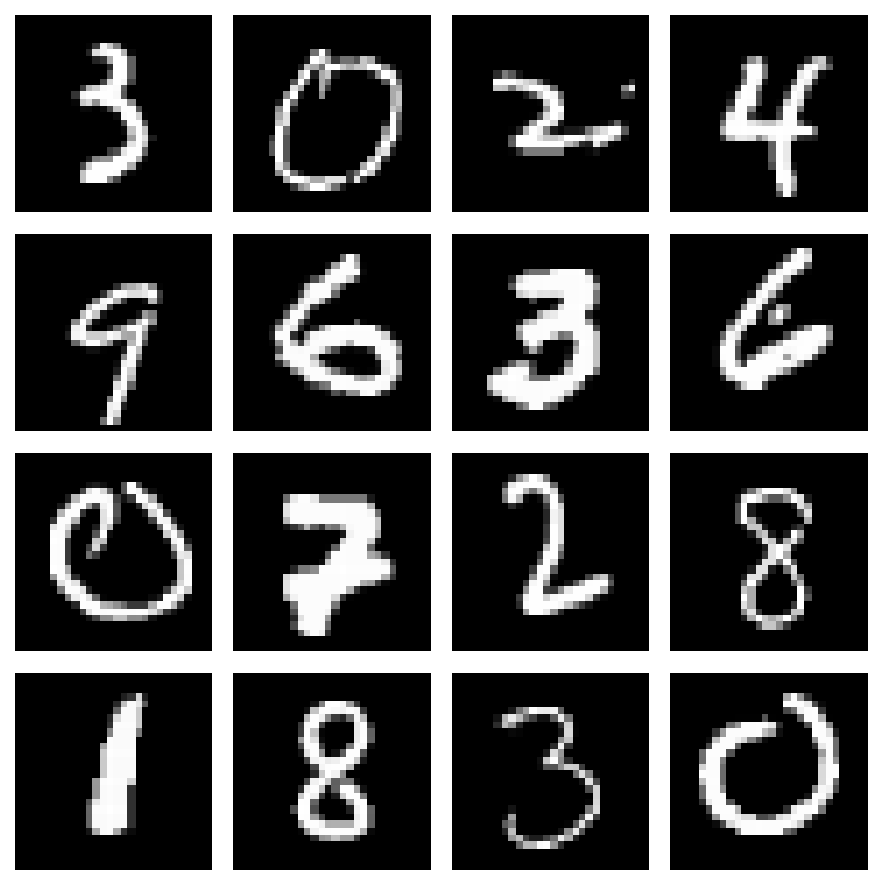
\includegraphics[width=.6\linewidth]{images/mnist.pdf}
      \caption{Random selection of images taken from the MNIST dataset \cite{bib:mnist}. The MNIST dataset consists of 28x28 grayscale images of handwritten digits from 0-9 and has 60000 training examples and 10000 testing examples.}
\label{fig:mnist}
\end{figure}
\FloatBarrier

\begin{figure}[!htb]
    \centering
  \begin{minipage}[b]{.48\linewidth}
      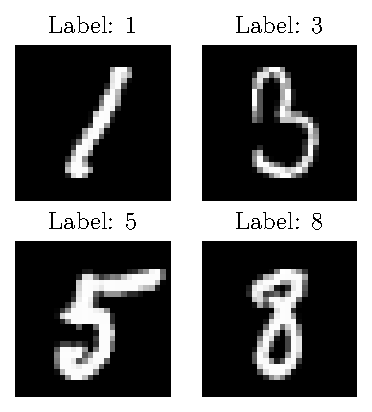
\includegraphics[width=\linewidth]{images/mnist_raw.pdf}
      \subcaption{Original.}
      \label{fig:mnist_dataset_original}
  \end{minipage}
  \begin{minipage}[b]{.48\linewidth}
      
\includegraphics[width=\linewidth]{images/mnist_binarized.pdf}
      \subcaption{Binarized.}
      \label{fig:mnist_dataset_binarized}
  \end{minipage}
  \caption{Part of sample from the original (\subref{fig:mnist_dataset_original}) and binarized (\subref{fig:mnist_dataset_binarized}) MNIST dataset. The original image is the number three and here we show a zoomed-in version(the upper right corner) to make the binarization visible. A LUT network can only do binary classification, so we have to binarize the labels as well. Numbers from 0-4 get the label 0 and numbers from 5-9 get the label 1.}
\label{fig:mnist_dataset}
\end{figure}
\FloatBarrier

\subsection{Experiments from paper}
We construct a LUT network with five hidden layers and 1024 LUTs per hidden layer. Every LUT in the network takes eight bits as input. Construction of the network is performed using the training set with 60000 samples and after training we validate on the test set with 10000 samples. The code is written by ourselves in Python using the package Numpy \cite{bib:harris2020array} for matrix operations. Similar to other machine learning packages, a LUT network object with provided arguments is first created and methods like \hl{\texttt{.train()}} and \hl{\texttt{.predict()}} allows the user to work with the LUT network at a high level. The code is available on GitHub \cite{bib:lut_github}. We obtain a training accuracy of 0.89 and a test accuracy of 0.87 which are the exact results from \cite{bib:chatterjee2018learning}. Note that the results are way above 0.5 meaning some learning had taken place. The way the LUT network is defined, every individual LUT already gives a prediction on the example passed to the network. That means we can compute the accuracy of every LUT in the network. Figure~\ref{fig:ex1_depth_performance} visualizes the training accuracy dependent on the layer. Each point represents the mean training accuracy over the respective layer and the total height of the error bars are two standard deviations. We can see that with increasing layer number, the accuracy goes up and the standard deviation goes down until it reaches zero at layer six because there is only one LUT in the last layer. Increasing performance with increasing depth reminds us of neural networks where adding more layers is a heuristic to increase performance.

\begin{figure}[!htb]
    \centering
    \includestandalone[]{standalone/lut/depth_performance}
    \caption{Training accuracy dependent on the layer for an 8-LUT network with five hidden layers (six is the output layer with just one LUT) and 1024 LUTs per hidden layer, trained on the Binary-MNIST dataset using our own code \cite{bib:lut_github}. The points represent the mean over the respective layer with two standard deviations as total height of the error bars. Similar to neural networks, we can see that performance increases with increasing depth. These results are our own and are almost identical to \cite{bib:chatterjee2018learning}.}
\label{fig:ex1_depth_performance}
\end{figure}
\FloatBarrier

\noindent The bit-size of the LUTs (denoted by $\delta$ in Algorithm~\ref{alg:LUT}) is a crucial hyperparameter. In another experiment, \cite{bib:chatterjee2018learning} varies the bit-size from two to 16 with steps of two and observes the effect on training and testing accuracy. The rest of the LUT network is the same as before. Figure~\ref{fig:ex1_k_acc} visualizes the results.

\begin{figure}[!htb]
    \centering
    \includestandalone[]{standalone/lut/k_acc_real}
    \caption{Training and testing accuracy on Binary-MNIST when the bit-size of a LUT newtwork with five hidden layers and 1024 LUT per hidden layer is varied. Increasing the bit-size sufficiently drives the training accuracy near perfection. As with machine learning models in general, the testing accuracy goes down with too much complexity, meaning we are overfitting. The underlying data to produce this plot is taken from \cite{bib:chatterjee2018learning}.}
\label{fig:ex1_k_acc}
\end{figure}
\FloatBarrier

\subsection{Varying the number of LUTs per hidden layer} \label{sec:num_luts_per_layer}
Throughout this thesis, we will stick with LUT networks with five hidden layers and 1024 LUTs per hidden layer to stay consistent with \cite{bib:chatterjee2018learning}. We will now invesigate what effect changing only the number of LUTs per hidden layer has. We use an 8-LUT network with five hidden layers and evaluate the accuracy at $2^i$ LUTs per layer, where $i = 1, \dots, 12$. The result can be seen in Figure~\ref{fig:num_luts_per_layer}, where Figure~\ref{fig:num_luts_per_layer:num} has an arithmetic scale and Figure~\ref{fig:num_luts_per_layer:num_log} has a logarithmic scale. We can see that going above 512 LUTs per hidden layer does not increase the accuracy anymore. In Section~\ref{sec:lut_network_size} we have seen that the number of LUTs per hidden layer is linearly proportional to the LUT network size on disk. So although not as important as the bit-size, which influences the LUT network size exponentially, reducing the number of LUTs per hidden layer seems like a quick and easy way to reduce LUT network size, especially if the performance does not drop.

\begin{figure}[!htb]
    \centering
  \begin{minipage}[b]{.45\linewidth}
    \resizebox {1\textwidth} {!} {
    \includestandalone[]{standalone/lut/nlpl_num}
    }
    \subcaption{Arithmetic scale.}
    \label{fig:num_luts_per_layer:num}
  \end{minipage}
  \begin{minipage}[b]{.45\linewidth}
    \resizebox {1\textwidth} {!} {
    \includestandalone[]{standalone/lut/nlpl_num_log}
    }
    \subcaption{Logarithmic scale.}
    \label{fig:num_luts_per_layer:num_log}
  \end{minipage}
  \caption{Accuracy of an 8-LUT network with five hidden layers dependent on the number of LUTs per hidden layer, where (\subref{fig:num_luts_per_layer:num}) provides an arithmetic scale and (\ref{fig:num_luts_per_layer:num_log}) provides a logarithmic scale. Increasing the number of LUTs per hidden layer above 512 has no effect on the accuracy.}
\label{fig:num_luts_per_layer}
\end{figure}
\FloatBarrier

\section{Improving LUT-based architectures}

\subsection{Majority vote} \label{sec:majority_vote}
So far the final prediction came from a single LUT that takes its inputs from the last hidden layer. Considering the same architecture as in the previous section, the last hidden layer has 1024 LUTs. If the number of bits per LUT is eight, then for the final prediction only eight of all 1024 LUTs will be used. Since every LUT is trained with the same label vector $\bm{y}$, each of the 1024 LUTs could theoretically be used for a final prediction too. That motivates us to try a \textit{wisdom of the crowd} technique, a majority vote mechanism that takes into account the predictions of all LUTs in the last hidden layer. The prediction that occurs most often will be chosen as the final one. The complete scheme can be seen in Algorithm~\ref{alg:majority_vote}. We conduct an experiment using a LUT network with five hidden layers and 1024 LUTs per hidden layer, varying the bit-size from two to 10 with steps of one, predicting with and without majority vote each time. The result can be seen in Figure~\ref{fig:majority_vote}. We can see that for a low bit-size, using a majority vote significantly boosts the training and testing accuracy. For high bit-sizes, a majority vote has less effect, but still enhances the testing performance a little. Interestingly, at five bits per LUT all accuracies coincide. Since using a majority vote requires almost no extra computational effort and at worst the results stay the same, it seems to be a good technique for enhancing the network's performance.

\begin{algorithm}
  \caption{LUT network majority vote}
  \label{alg:majority_vote}
  \begin{algorithmic}
    \State Given binary vector $\bm{x}$ and trained LUT network according to Algorithm~\ref{alg:LUT} with $l_L$ LUTs in the last hidden layer, perform a majority vote to predict.
    \vspace{1em}
    \State Initialize empty list $\alpha = [\hspace{0.3em}]$
    \For{$i=1, \dots, j_L$}
      \State Append prediction of LUT$_i$ on $\bm{x}$ to $\alpha$ (either 0 or 1)
    \EndFor
    \If{$\sum\limits_{\alpha_i = 0} > \sum\limits_{\alpha_i = 1}$}
      \State Return 0
    \ElsIf{$\sum\limits_{\alpha_i = 0} < \sum\limits_{\alpha_i = 1}$}
      \State Return 1
    \Else
      \State Return random choice of $\{0, 1\}$
    \EndIf
  \end{algorithmic}
\end{algorithm}
\FloatBarrier

\begin{figure}[!htb]
    \centering
    \includestandalone[]{standalone/lut/majority_vote}
    \caption{Training and testing accuracies with and without using a majority vote mechanism for a LUT network with five hidden layers and 1024 LUTs per hidden layer. The task is Binary-MNIST. For low bit-sizes, using a majority vote significantly enhances performance while the effect lessens with higher bit-sizes, but still enhances the testing accuracy a little. Interestingly, all accuracies coincide at five LUTs per hidden layer.}
\label{fig:majority_vote}
\end{figure}
\FloatBarrier

\subsection{Maximizing layer-wise mean accuracy while training} \label{sec:max_layer_acc}
As mentioned earlier, every LUT is trained with the same label vector $\bm{y}$ and is able to give a prediction. With increasing hidden layer, the LUTs get increasingly better. Figure~\ref{fig:acc_layer_normal} visualizes this using histograms. The underlying data is the training accuracy per LUT per hidden layer for an 8-LUT network with five hidden layers and 1024 LUTs per hidden layer applied on the Binary-MNIST dataset. The training accuracy of this LUT network is 0.89 and the testing accuracy is 0.87, the same accuracies as in the first experiment. The $x$-axis represents the training accuracy. For each hidden layer, we divide the data in 10 equally-sized bins (in terms of the accuracy) from the minimum to maximum value. Then for each bin, we erect a bar, where the height represents the number of data points that fall into this bin. We can see that on average, the accuracy increases with hidden layer number and the spread of accuracies reduces dramatically. For hidden layer 1, the accuracies are worst and the spread is maximal. The worst LUTs on hidden layer 1 are only slightly better than chance. That motivates us to conduct an experiment in which we try to maximize the accuracy of the LUTs while training.

We conceptualize following algorithm: after training a layer, we discard the $n$ worst LUTs in that layer and establish $n$ new LUTs that are hopefully better. We said \enquote{hopefully} because the learning algorithm takes a random subset of columns of the previous layer, leaving it to chance if a new LUT will perform better in terms of accuracy. After obtaining those $n$ new LUTs, we score every LUT and again discard the $n$ worst LUTs until the mean accuracy does not change anymore. We set a patience $p$, i.e., a number of iterations after no change in mean accuracy we will move onto the next layer. The implementation is described in Algorithm~\ref{alg:max_layer_acc}.

\begin{figure}[!htb]
    \centering
    \includestandalone[]{standalone/lut/acc_layer_normal}
    \caption{Histograms of training accuracies per hidden layer for an 8-LUT network with five hidden layers and 1024 LUTs per hidden layer. The task is Binary-MNIST. For each hidden layer, the data is divided into 10 equally sized bins from minimum to maximum value. For each range, we erect a bar with the height equal to the number of data points that fall within that range. The overall accuracy of this network is 0.89 on the training set and 0.87 on the testing set.}
\label{fig:acc_layer_normal}
\end{figure}
\FloatBarrier

\begin{algorithm}
  \caption{Maximizing layer-wise mean accuracy while training}
  \label{alg:max_layer_acc}
  \begin{algorithmic}
    \State Given binary features $\bm{X}$ with $N$ rows and binary label vector $\bm{y}$, construct a LUT network with $L$ hidden layers where the training accuracy in each hidden layer is maximized. This algorithm modifies Algorithm~\ref{alg:LUT}.
    \vspace{1em}
    \State Choose additional hyperparameters:
    \Statein Number of LUTs $n$ to discard after each iteration
    \Statein Patience $p \in \mathds{N}$
    \For{$i = 1, \dots, L$}
      \State Train layer $L$ as in Algorithm~\ref{alg:LUT}
      \State $\text{no\_change} \in \mathds{N} \gets 0$
      \State $\text{best} \in \mathds{R} \gets 0$
      \While{$\text{no\_change} < p$}
      \State Discard $n$ worst performing LUTs on $(\bm{X}, \bm{y})$
      \State Append $n$ new LUTs trained on $(\bm{X}, \bm{y})$ to the current layer
        \State $\text{accs} \in \mathds{R}^N \gets $ accuracy of each LUT on $(\bm{X}, \bm{y})$
        \State $\text{curr} \in \mathds{R} \gets \text{mean}(\text{accs})$
        \If{$\text{curr} > \text{best}$}
          \State $\text{best} \gets \text{curr}$
          \State $\text{no\_change} \gets 0$
          \Else
            \State $\text{no\_change} \mathrel{+}= 1$
        \EndIf
      \EndWhile
    \EndFor
    \State The single LUT after the last hidden layer is created as usual
  \end{algorithmic}
\end{algorithm}
\FloatBarrier

\noindent Starting another experiment, we again use an 8-LUT network with five hidden layers and 1024 LUTs per hidden layer and the Binary-MNIST dataset. We set $p=10$ and $n=50$. After running Algorithm~\ref{alg:max_layer_acc}, we obtain a training accuracy of 0.90 and a testing accuracy of 0.88, slightly better than before. In Figure~\ref{fig:acc_layer_discard} we can see the accuracies per hidden layer visualized using a histogram. Contrary to Figure~\ref{fig:acc_layer_normal}, the distributions are much more narrow now. After training we also tried prediction with a majority vote, but the accuracies did not change.

\begin{figure}[!htb]
    \centering
    \includestandalone[]{standalone/lut/acc_layer_discard}
    \caption{Histograms of training accuracies per hidden layer for an 8-LUT network with five hidden layers and 1024 LUTs per hidden layer, applied on Binary-MNIST. For this network, we applied Algorithm~\ref{alg:max_layer_acc} to try to improve performance, yielding an overall accuracy of 0.90 on the training set and 0.88 on the testing set. The results of this network are slightly better (increase of 1\% training and testing accuracy) compared to the same network without optimization. Contrary to Figure~\ref{fig:acc_layer_normal}, the distributions are much narrower.}
\label{fig:acc_layer_discard}
\end{figure}
\FloatBarrier

\noindent For a more complete picture, we vary the bit-size from two to 10 while applying Algorithm~\ref{alg:max_layer_acc}. There are again five hidden layers with 1024 LUTs per hidden layer. The result can be seen in Figure~\ref{fig:increase_layer_acc}. We can see that pushing up the layer-wise accuracy does indeed help increase the overall accuracy, albeit only significantly for low bit-sizes. For high bit-sizes, the effect is diminished.


\begin{figure}[!htb]
    \centering
    \includestandalone[]{standalone/lut/increase_layer_acc}
    \caption{Training and testing accuracies for LUT networks of varying bit-size with five layers and 1024 LUTs per hidden layer applied on Binary-MNIST. Solid lines and markers denote accuracies of networks where we applied Algorithm~\ref{alg:max_layer_acc}. For low bit-sizes, improving the layer-wise accuracies has a significant effect on the overall performance, while for higher bit-sizes the effect is diminished.}
\label{fig:increase_layer_acc}
\end{figure}
\FloatBarrier

\subsection{Feature engineering} \label{sec:feature_engineering}
So far we have not done any more sophisticated feature engineering except making a binary version out of the original MNIST dataset. Since feature engineering is an integral part of machine learning in general, we try it too and see if there is an improvement of the model's performance. We enhance the data by emphasizing the edges. Concretely, we create a copy of the original image and replace each pixel with black if the adjacent pixel has the same value and white if the adjacent pixel has a different value. We do this process both in $x$- and $y$-direction and add the results to the original image. Figure~\ref{fig:sobel_single} illustrates this technique for one example.

\begin{figure}[!htb]
    \centering
    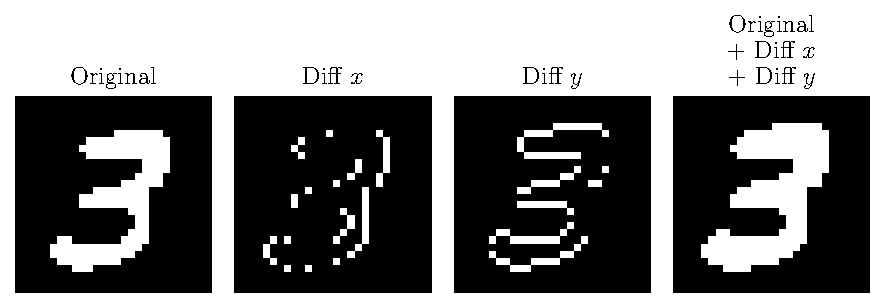
\includegraphics[width=.9\linewidth]{images/diff.pdf}
    \caption{Single example from the training data where we applied feature engineering. We create a copy of the original image and replace each pixel with black if the adjacent pixel has the same value and white if the adjacent pixel has a different value. We perform this process both in $x$- and $y$-direction and add the results to the original image. Looking at the feature-engineered image on the right, the number appears thicker.}
\label{fig:sobel_single}
\end{figure}
\FloatBarrier

\noindent Using the dataset enhanced with feature engineering, we train a LUT network with five hidden layers and 1024 LUTs per hidden layer, varying the bit-size from two to 10. The result can be seen in Figure~\ref{fig:sobel_acc}. We can see that the accuracies are consistently higher for models that were trained on images where feature engineering had been applied. The technique described in this section was inspired by the Sobel operator \cite{bib:sobelsobel} which calculates the gradients in an image in either $x$- or $y$-direction. Using this operator as feature engineering technique as opposed to our own produces similar results. We presented our own as main technique for the sake of an easier explanation and brevity.

\begin{figure}[!htb]
    \centering
    \includestandalone[]{standalone/lut/feature_engineering}
    \caption{Train and test accuracies for models trained on unmodified Binary-MNIST data and Binary-MNIST data where feature engineering had been applied. We can see that using feature engineering boosts the performance slightly.}
\label{fig:sobel_acc}
\end{figure}
\FloatBarrier


\subsection{Plain LUT ensembling} \label{sec:plain_lut_ensemble}
In Section~\ref{sec:majority_vote}, as opposed to having one final LUT, we counted the number of output labels in the last hidden layer and took that label as final prediction whichever was occurring the most. We could view that as a \textit{wisdom of the crowd} technique. Another approach is to bunch together $n$ separate LUT networks that do not use a majority vote and combine their prediction into one. We simply use that label as final prediction which was predicted the most out of the $n$ LUT networks. In the event that both labels occur the same number of times, we make a random choice. The scheme is described in detail in Algorithm~\ref{alg:lut_ensemble}.

We conduct an ensembling experiment where we use 2-LUTs as base classifiers. Keeping the bit-size low allows us to increase the number of individual LUT networks to a much higher degree. Training and inference for 8-LUT networks would take too long, at least with our current code. Figure~\ref{fig:plain_lut_ensembling} visualizes the result of the experiment. We use LUT network ensembles with $2^{1, \dots, 10}$ individual LUT classifiers. At just two LUT networks, the training accuracy is fairly low at 0.68, as it would be with a single 2-LUT network. Increasing the number of LUT networks increases the training accuracy and a peak at 0.78 with 64 LUTs is reached. Increasing the number of LUTs even more has no effect on the accuracy. Interestingly, the testing accuracy is consistently higher than the training accuracy.

\begin{algorithm}
  \caption{LUT ensembling}
  \label{alg:lut_ensemble}
  \begin{algorithmic}
    \State Given trained $\text{LUT}_{1, \dots, n}$, perform ensembling to predict on yet unseen $\bm{x}$.
    \vspace{1em}
    \State Initialize empty list $\alpha = [\hspace{0.3em}]$
    \For{$i=1, \dots, n$}
      \State Append prediction of LUT$_i$ on $\bm{x}$ to $\alpha$ (either 0 or 1)
    \EndFor
    \If{$\sum\limits_{\alpha_i = 0} > \sum\limits_{\alpha_i = 1}$}
      \State Return 0
    \ElsIf{$\sum\limits_{\alpha_i = 0} < \sum\limits_{\alpha_i = 1}$}
      \State Return 1
    \Else
      \State Return random choice of $\{0, 1\}$
    \EndIf
  \end{algorithmic}
\end{algorithm}
\FloatBarrier

\begin{figure}[!htb]
    \centering
    \includestandalone[]{standalone/lut/plain_lut_ensembling}
    \caption{Train and test accuracies for LUT network ensembles according to Algorithm~\ref{alg:lut_ensemble} on Binary-MNIST. The base classifiers are 2-LUT networks with five hidden layers and 1024 LUTs per hidden layer. Training and testing accuracies reach a peak at 64 LUT networks, increasing the LUT number even more has no effect on the accuracy. Interestingly, the testing accuracy is consistently higher than the training accuracy.}
\label{fig:plain_lut_ensembling}
\end{figure}
\FloatBarrier

\subsection{Advanced LUT ensembling} \label{sec:ada_boost}
Now we try another ensembling method which is very well established in literature and practice, the AdaBoost.M1 algorithm \cite{bib:adaboostm1} which can be seen in Algorithm~\ref{alg:adaboostm1}. As the scheme in the previous Section~\ref{sec:plain_lut_ensemble}, AdaBoost.M1 combines predictions of $n$ separate classifiers $f_{1, \dots, n}$ into one. Every classifier is trained individually with the addition of weights $\bm{w}$, where $w_k > 0$. Every sample $k$ in the training set is assigned weight $w_k = 1/N$ in the beginning, where $N$ is the number of samples. The weights represent how much attention during training a single example should get, the higher the weight, the more attention the sample gets. Since all weights are equal in the beginning, every sample gets the same amount of attention in the first iteration. Once iteration $i$ is finished, a number $\alpha_i \in \mathds{R}$ is computed. If $\alpha_i > 0$, then the classifier is better than random and if $\alpha_i < 0$, then the classifier is worse than random. Using $\alpha_i$, we update each weight of only those samples which were misclassified. If the classifier is better than random, then we can do some fine-tuning and focus more on the misclassifications which corresponds to assigning higher weights to misclassified samples. If the classifier is worse than random, then we are not yet ready for fine-tuning and we should focus more on the most important samples which corresponds to assigning lower weights to misclassified samples. After $n$ iterations, training is finished and we can predict on yet unseen sample $\bm{x}$ using $\text{sign}(\sum_{i=1}^n \alpha_i f_i(\bm{x}))$. 

\begin{algorithm}
  \caption{AdaBoost.M1 algorithm according to \cite{bib:adaboostm1}} \label{alg:adaboostm1}
  \begin{algorithmic}[1]
    \State Given dataset $(\bm{X}, \bm{y})$, where $\bm{X} = \bm{x}_1, \dots, \bm{x}_N$ and $\bm{y} = y_1, \dots, y_N$, $y_i \in \{-1, 1\}$ and model class, construct a classifier that is made up of $n$ individual classifiers $f_1, \dots, f_n$.
    \vspace{1em}
    \State Initialize weight vector $\bm{w} \in \mathds{R}^N$ with $w_{1, \dots, N} = 1/N$
    \vspace{0.5em}
    \For{$i = 1, \dots, n$}
    \State Train classifier $f_i$ on $(\bm{X},\bm{y})$ and weights $\bm{w}$ \label{alg_line:adaboostm1:train}
    \State $\text{err}_i \gets \big( \sum_{k=1}^N w_k \mathbb{1}(f_i(\bm{x}_k) \neq y_k) \big) / \sum_{k=1}^N w_k$
    \State $\alpha_i = \log((1 - \text{err}_i) / \text{err}_i)$
    \For{$k = 1, \dots, N$}
    \State $w_k \gets w_k \exp(\alpha_i \mathbb{1}(f_i(\bm{x}_k) \neq y_k))$
    \EndFor
    \EndFor
    \State Prediction on yet unseen $\bm{x}$: $\text{sign} \big( \sum_{i = 1}^n \alpha_i f_i(\bm{x}) \big)$
  \end{algorithmic}
\end{algorithm}
\FloatBarrier

\noindent Using AdaBoost.M1 with LUT networks only works if we modify the algorithm slightly. Looking at Algorithm~\ref{alg:adaboostm1} on line~\ref{alg_line:adaboostm1:train}, we notice that there is no way to incorporate weights into the LUT learning algorithm (see Algorithm~\ref{alg:LUT}). Therefore, instead of training on all samples $\bm{X}$ with weights at each iteration, we train on a subset of samples $\bm{X}' \subset \bm{X}$ with fixed size $\rho \in \{1, \dots, N\}$ without weights. By choosing those samples with highest weights to be included in $\bm{X}'$, we are able to give more attention to those samples. The modified AdaBoost.M1 for LUT networks can be seen in Algorithm~\ref{alg:lut_ensemble_ada}. The modifications take place from line~\ref{alg_ref:lut_ensemble_ada:mod_begin} to line~\ref{alg_ref:lut_ensemble_ada:mod_end}. On the first iteration, we train on the entire dataset. On all other iterations, we train on $\rho$ samples with the highest weights. The command $\text{argsort}(\bm{w})$ returns indices that would sort $\bm{w}$. We are interested in the highest weights, not the lowest ones, so we reverse the sorted indices: $\text{reversed}(\text{argsort}(\bm{w}))$. We then take a subset, the first $\rho$ entries: $\text{reversed}(\text{argsort}(\bm{w}))[:\rho]$. Now we have the indices of $\rho$ samples with highest weights and take a subset of the dataset: $\bm{X}[\text{idxs}]$ and $\bm{y}[\text{idxs}]$.

\begin{algorithm}
  \caption{LUT ensembling inspired by AdaBoost.M1}\label{alg:lut_ensemble_ada}
  \begin{algorithmic}[1]
    \State Given dataset $(\bm{X}, \bm{y})$, where $\bm{X} = \bm{x}_1, \dots, \bm{x}_N$ and $\bm{y} = y_1, \dots, y_N$, $y_i \in \{-1, 1\}$, construct a classifier that is made up of $n$ individual classifiers $\text{LUT}_{1, \dots, n}$.
    \vspace{1em}
    \State Initialize weight vector $\bm{w} \in \mathds{R}^N$ with $w_{1, \dots, N} = 1/N$
    \State Choose $\rho$ out of $\{1, \dots, N\}$
    \vspace{0.5em}
    \For{$i = 1, \dots, n$} \label{alg_ref:lut_ensemble_ada:mod_begin}
    \If{i = 1}
      \State Train $\text{LUT}_i$ on $(\bm{X},\bm{y})$
    \Else
    \State $\text{idxs} = \text{reversed}(\text{argsort}(\bm{w}))[:\rho]$
    \State $\bm{X}' \subset \bm{X} \gets \bm{X}[\text{idxs}]$
    \State $\bm{y}' \subset \bm{y} \gets \bm{y}[\text{idxs}]$
      \State Train $\text{LUT}_i$ on $(\bm{X}', \bm{y}')$
      \EndIf \label{alg_ref:lut_ensemble_ada:mod_end}
    \State $\text{err}_i \gets \big( \sum_{k=1}^N w_k \mathbb{1}(\text{LUT}_i(\bm{x}_k) \neq y_k) \big) / \sum_{k=1}^N w_k$
    \State $\alpha_i = \log((1 - \text{err}_i) / \text{err}_i)$
    \For{$k = 1, \dots, N$}
    \State $w_k \gets w_k \exp(\alpha_i \mathbb{1}(\text{LUT}_i(\bm{x}_k) \neq y_k))$
    \EndFor
    \EndFor
    \State Prediction on yet unseen $\bm{x}$: $\text{sign} \big( \sum_{i = 1}^n \alpha_i \text{LUT}_i(\bm{x}) \big)$
  \end{algorithmic}
\end{algorithm}
\FloatBarrier

\noindent We apply Algorithm~\ref{alg:lut_ensemble_ada} and use 2-LUT networks with five hidden layers and 1024 LUTs per hidden layer and choose $\rho = N/5$. We vary the number of LUT networks from 2 to 1024. The motivation for choosing 2-LUT networks is computation time and disk size. Since we want to keep open the possibility for many LUT networks in the ensembled classifier, we have to restrict ourselves with the bit-size, otherwise it would take too long to train and predict. Our overall goal also includes a small disk size. A LUT network ensemble of 8-LUTs with five hidden layers and 1024 LUTS per hidden layer would take up 168 MB of space, way out of proportions. The results can be seen in Figure~\ref{fig:ada_2_LUT}. We can see that with an increasing number of LUT networks, we can indeed improve the accuracy. At 1024 LUT networks, we achieve a training accuracy of 0.94 and testing accuracy of 0.93. When it comes to the testing accuracy, this is the best result so far. Interesting is the lack of a significant difference between training and testing accuracies. Usually there is a point where overfitting starts to take place and the testing accuracy decreases compared to the training accuracy. Perhaps overfitting will take place at more LUT networks than 1024, but we do not go above that because it would take too much time to train for us. However, a LUT network ensemble of 2-LUTs with five hidden layers and 1024 LUTs per hidden layer takes up 2.62 MB of disk space, larger than the CNN we used before which was 1.16 MB in size. We therefore evaluate training and testing performance on a 2-LUT ensemble with five hidden layers and only 64 LUTs per hidden layer. This architecture takes up only 168 KB of disk space. We obtain a trainig and testing accuracy of 0.94.

\begin{figure}[!htb]
    \centering
    \includestandalone[]{standalone/lut/ada_2_LUT}
    \caption{Training and testing accuracies for ensembles of 2-LUT networks with five hidden layers and 1024 LUTs per hidden layer according to Algorithm~\ref{alg:lut_ensemble_ada}. At 1024 LUT networks, we obtain training and testing accuracies of 0.94 and 0.93, respectively, best so far when it comes to testing accuracy. Notice the lack of significant difference between training and testing accuracy as it would be when overfitting. Perhaps overfitting takes place at more individual LUTs. Using 1024 LUT networks per hidden layer make the size of this ensemble be 2.62 MB which is bigger than the CNN with 1.16 MB we used before. Performing another experiment with an ensemble of 1024 2-LUT networks with five hidden layers and only 64 LUTs per hidden layer, we obtain a training and testing accuracy of 0.94 and this architecture only takes up 168 KB of space.}
\label{fig:ada_2_LUT}
\end{figure}
\FloatBarrier

\subsection{Combining different methods}
We combine different methods presented in previous sections to try to push the accuracies even further. We utilize an AdaBoost.M1 inspired LUT classifier from Section~\ref{sec:ada_boost} with 1024 individual 2-LUT networks that each have 5 hidden layers and 64 LUTs per hidden layer. Additionally, we apply Algorithm~\ref{alg:max_layer_acc} to each LUT network while training and also use the feature-engineered dataset from Section~\ref{sec:feature_engineering}. For the hyperparameters, we set $\rho = N/5$, the number of LUTs to discard after each iteration $n=10$ and patience $p=10$. We obtain a training accuracy of 0.75 and testing accuracy of 0.78, worse than the results from Section~\ref{sec:ada_boost}. The results make us question Algorithm~\ref{alg:max_layer_acc}. It is interesting though that pushing up the accuracies of individual LUTs in LUT networks leads to an overall inferior performance when constructing an ensembled classifier.

\subsection{Findings and limitations, recommendations, future work}
We introduced the concept of LUTs from \cite{bib:chatterjee2018learning}, recreated results from the paper and consequently tried to improve LUT-based architectures by inventing new schemes. We were able to improve performance significantly in Section~\ref{sec:ada_boost}, not to the extent to a convolutional neural network, but perhaps with more research, the performance of LUT-based models can be increased even further. When it comes to model size, the bit-size is crucial. Since the size of a LUT table is exponentially proportional to the bit-size, a too large bit size quickly increases size on disk with questionable improvement in performance, see Section~\ref{sec:models}. As we have seen in Section~\ref{sec:num_luts_per_layer}, we can significantly decrease the number of LUTs per hidden layer in a LUT network without much loss of accuracy. Making a good choice of architecture, combined with ensembling techniques results in LUT-based models that are comparitively small and have boosted accuracy. Lastly, since LUTs do not require floating-point operations, they have the potential for really fast implementations, possibly even on hardware. What we have not discussed is pruning of LUT networks, i.e. discarding individual LUTs that do nothing.  After all, we have seen in Section~\ref{sec:luts} that it is possible that individual LUTs in a LUT network do not contribute to the final prediction. We have also not discussed multi-class classification which would be possible with LUTs using an one-vs-one or one-vs-all approach similar to SVMs \cite{bib:bishop2006pattern}.
